\chapter{The Oscilloscope}

\section{Introduction}

The cathode ray oscilloscope, one of the most useful tools in modern experimental physics, can measure potential differences which change rapidly with time -- too rapidly to be followed by the needle of a simple voltmeter (some examples are shown in figure \ref{fig:voltagesample} below). You are encouraged to explore the operation of the oscilloscope by manipulating all of the controls.

\begin{figure}[h]
    \begin{center}
        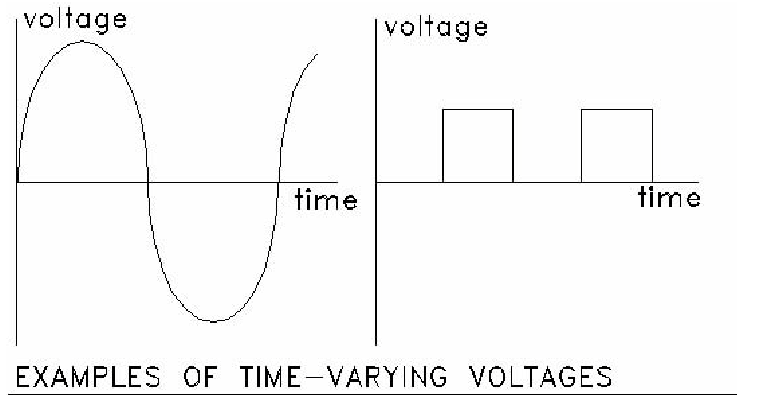
\includegraphics[width=0.6\textwidth]{./Exp3/pic/image1.png}
    \end{center}
    \caption{Examples of Time-varying Voltages}
    \label{fig:voltagesample}
\end{figure}

\subsection{The Cathode Ray Tube}

Figure \ref{fig:cathodtube} shows schematically the essential features of the cathode ray tube in the oscilloscope. The cathode ray tube is the fundamental component of the oscilloscope; in it the electron beam is deflected based on the potential difference that we are trying to measure. The electron beam is then incident on a fluorescent screen which allows us to see the results of the deflection caused by the potential difference. \myskip

\begin{figure}[h]
    \begin{center}
        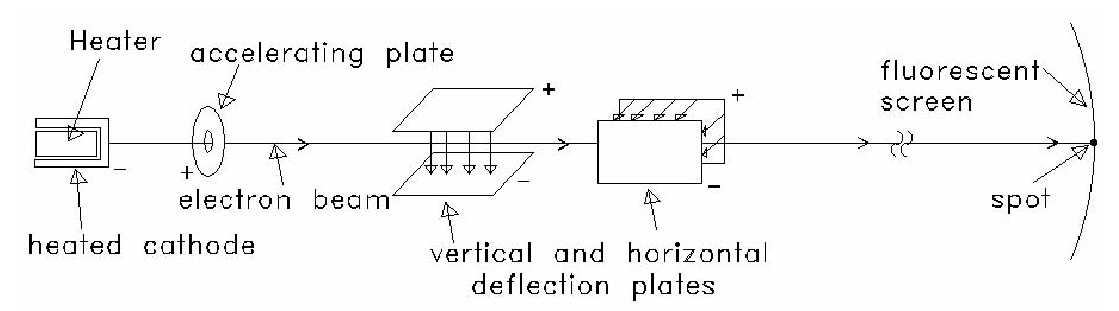
\includegraphics[width=0.9\textwidth]{./Exp3/pic/image2.png}
    \end{center}
    \caption{Schematic Diagram of a Cathode Ray Tube}
    \label{fig:cathodtube}
\end{figure}


Electrons leave the \textbf{heated cathode}, are accelerated through a fixed voltage, and emerge as a narrow beam focused through a hole in the \textbf{accelerating plate}. When the \textbf{electron beam} strikes the \textbf{fluorescent screen} on the face of the tube, it produces a small luminous spot. Between the accelerating plate and the screen are two pairs of parallel deflection plates -- vertical and horizontal. A potential difference can be measured by applying it across one of these pairs of deflection plates. Before the potential difference is applied to either of these plate pairs it passes through a \textbf{vertical} or \textbf{horiztonal amplifier} to increase the voltage of the signal. The applied potential difference results in a transverse uniform electric field between the plates, by which the beam is then deflected. The direction of the deflection (up-down or left-right) is determined by which of the two pairs of deflecting plates (vertical or horizontal) the voltage is applied to. Usually, the potential difference we are interested in measuring is applied to the vertical deflection plates. \myskip

The applied potential is directly proportional to:
\begin{enumerate}
    \item the electric field strength between the plates $\left( V = E\cdot d \right)$
    \item the transverse force on the electrons $\left( E = F /q \right)$
    \item the resultant transverse acceleration of the electrons $\left( F = ma \right)$
\end{enumerate}
and since the time to travel the length of the plates does not depend on the transverse force, it is also directly proportional to:
\begin{enumerate}
    \setcounter{enumi}{3}
    \item the net transverse displacement of the electrons $\displaystyle\left( x = \frac{1}{2}at^2;\ t=\text{const},\ v_0=0 \right)$
    \item the transverse component of their velocity $\left( v = at;\ t=\text{const},\ v_0 = 0 \right)$
    \item the tangent of the angle at which the beam leaves the region between the plates $\displaystyle \left( \tan\theta = \frac{v_\text{transverse}}{v_\text{parallel}};\ v_\text{parallel} = \text{const} \right)$
\end{enumerate}

Therefore, when any of these quantities are multiplied by any factor, all of the others are multiplied by the same factor. \myskip

The net displacement of the spot on the screen will therefore be proportional to the applied potential difference. Therefore, by viewing the image on the oscilloscope, one can determine the voltage applied to the plates.

\subsection{Display of Time-Varying Potential Difference}

\begin{figure}[h]
    \begin{center}
        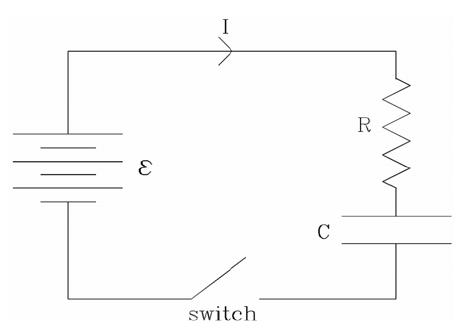
\includegraphics[width=0.3\textwidth]{./Exp3/pic/image3.png}
    \end{center}
    \caption{Horizontal Sweep Voltage}
    \label{fig:horizvol}
\end{figure}

In order to display the time variation of a potential difference which is applied across the \textbf{vertical deflection plates}, the beam can be deflected horizontally by an internally-generated voltage which increases uniformly with time. Figure \ref{fig:horizvol} indicates the ``sawtooth'' voltage which, when applied to the \textbf{horizontal deflection plates}, sweeps the beam \emph{horizontally} across the screen at \emph{constant velocity}, and returns the beam to its initial position and repeats the sweep, etc. \myskip

\begin{figure}[h]
    \begin{center}
        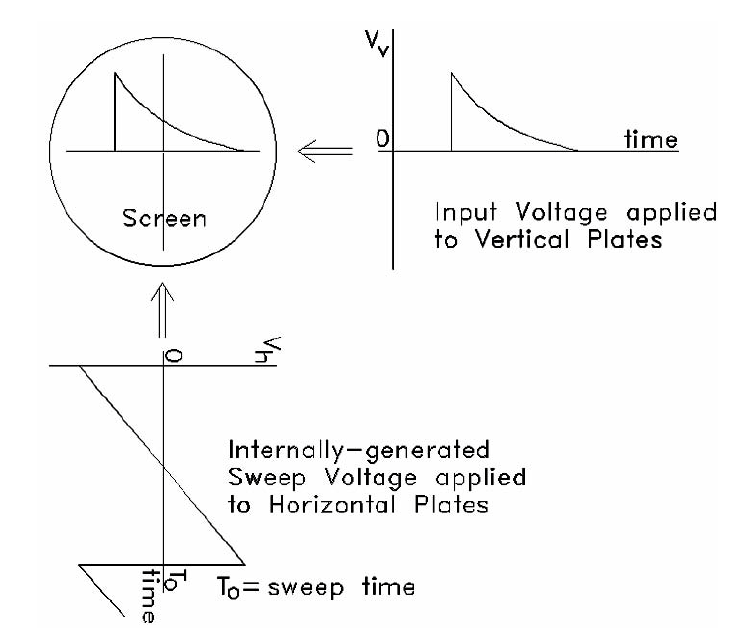
\includegraphics[width=0.6\textwidth]{./Exp3/pic/image4.png}
    \end{center}
    \caption{The image on the screen is formed by combining the constant horizontal sweep with a vertical deflection proportional to some time-dependent input voltage which you want to observe.}
    \label{fig:vertsweep}
\end{figure}

The process is somewhat similar to writing on paper. To write, one ``wiggles'' the pen up and down while moving the hand horizontally across the paper. Here the time-varying voltage applied to the vertical plates ``wiggles'' the electron beam up and down while the linear sweep voltage moves the beam horizontally with constant velocity (See figure \ref{fig:vertsweep}). The beam leaves its written trace on the tube screen. The motion in the vertical plane therefore usually corresponds to the voltage we are measuring, while the motion in the horizontal plane usually corresponds to the passage of time. \myskip

Because of the persistence of vision (approximately 0.05 sec) and because of the screen fluorescence, we see a plot of the potential as a function of time displayed on the screen.  \myskip

Usually one observes the repeating pattern of a periodically varying voltage by appropriate adjustment of the sweep time and synchronization of the start of successive sweeps. Oscilloscope controls allow one to determine when the sweep begins (on the oscilloscope this is called the ``trigger''). See the description of the horizontal sweep trigger controls (17-21) in the instructions for the oscilloscope in the next section.

\newpage
\section{The Oscilloscope}

\begin{figure}[h]
    \begin{center}
        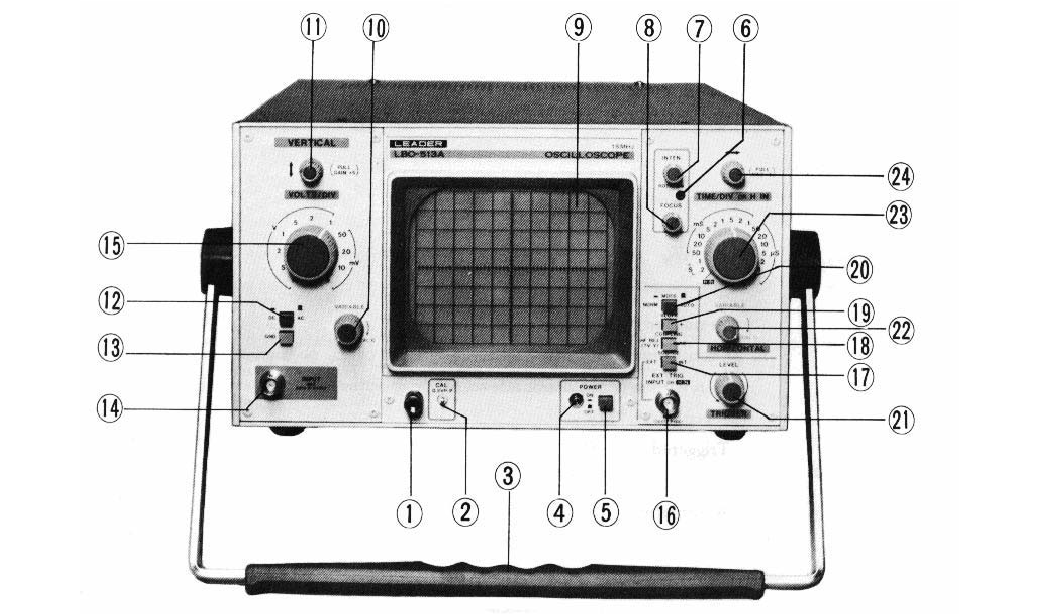
\includegraphics[width=0.9\textwidth]{./Exp3/pic/imageosc.png}
    \end{center}
    \caption{Leader Model LBO-513A Oscilloscope}
    \label{fig:oscillofront}
\end{figure}

The front panel of the Leader Model LBO - 513A oscilloscope is shown in the figure \ref{fig:oscillofront}. The inputs and controls with which you will be concerned can be divided into three groups depending on the part of the oscilloscope circuitry with which they are associated. All oscilloscopes include this basic set of controls. The numbers in the diagram refer to the controls described below. \myskip

\subsection{FORMATION OF THE ELECTRON BEAM}

\indent \indent (5) \textbf{POWER}\myskip

\indent \indent Push in to turn the power on.\myskip

\indent (7) BEAM \textbf{INTEN}SITY \myskip

\indent \indent The \textbf{INTEN} control adjusts the intensity or brightness of the trace. Clockwise rotation increases the intensity. \myskip

\indent \textbf{NOTE}: When the spot on the screen is stationary, keep the intensity very low in order not to damage the fluorescent screen at that point. In general, do not leave the intensity higher than necessary for reasonable visibility. \myskip

\indent (8) BEAM \textbf{FOCUS} \myskip

\indent \indent The \textbf{FOCUS} control adjusts the sharpness of the electron spot on the screen.

\subsection{VERTICAL DEFLECTION OF THE ELECTRON BEAM}

\indent \indent (10) VERTICAL AXIS SENSITIVITY: \textbf{VARIABLE} FINE ADJUSTMENT. \myskip

\indent \indent The vertical axis \textbf{VARIABLE} control is used for fine adjustments of the vertical axis sensitivity. The sensitivity is reduced by turning the vertical axis \textbf{VARIABLE} knob counterclockwise. \myskip

\indent \indent In the fully clockwise position (with the knob clicked into this position) quantitative data about the potential difference can be read from the \textbf{VOLTS/DIV} setting. \myskip

\indent (15) VERTICAL AXIS SENSITIVITY: RANGE SELECTION IN VOLTS/DIV.\myskip 

\indent \indent The \textbf{VOLTS/DIV} 11-position switch determines the sensitivity of the vertical amplifier. The 11 ranges are indicated in volts per division on the front panel. \myskip

\indent \indent The indicated sensitivities are only correct if the vertical axis \textbf{VARIABLE} control is in the calibrated position (fully clockwise -- see (10)) and the \textbf{VERTICAL} position control is pushed in (the Gain = 1 position -- see (11-B)).\myskip

\indent (11-A) \textbf{VERTICAL} POSITION: \myskip

\indent \indent This control is used to move the displayed trace up or down. Turning the knob clockwise moves the trace upward.\myskip

\indent (11-B) VERTICAL AXIS MAGNIFIER: \textbf{GAIN $\times$ 5}:\myskip

\indent \indent If the \textbf{VERTICAL} position control is pulled out, the vertical axis sensitivity is increased by a factor of 5.\myskip

\indent (12) \textbf{AC-DC} INPUT SELECTOR:\myskip

\indent \indent AC stands for ``alternating current,'' a current that changes with time, while DC stands for ``direct current,'' a current that is constant in time.\myskip

\indent \indent With the button in (DC position), the input terminal is directly coupled to the vertical amplifier and both AC and DC signals are shown. With the button out (AC position) the DC signal is blocked by a capacitor so only the AC, or varying, signal is shown while the DC, or constant, signal is subtracted off. \myskip

\indent (13) \textbf{GND} GROUND SWITCH:\myskip

\indent \indent With the \textbf{GND} button in, the input to the vertical amplifier is grounded and therefore there is no deflection in the vertical direction.\myskip

\indent (14) VERTICAL \textbf{INPUT}: \myskip

\indent \indent This is the input terminal for the vertical amplifier. The maximum permissible input voltage is 600 Volts.

\subsection{HORIZONTAL DEFLECTION OF THE ELECTRON BEAM}

\indent (16) \textbf{EXT TRIG INPUT} \emph{or} \textbf{H IN}: EXTERNAL TRIGGER INPUT OR HORIZONTAL INPUT: \myskip

\indent \indent This input is used for externally triggering the horizontal sweep or for the HORIZONTAL INPUT in an x-y plot. This input is DC coupled (either a constant or a time varying voltage may be used -- compare with (12) above) and the maximum allowable applied voltage is 100 volts.\myskip

\indent (17-21) HORIZONTAL SWEEP TRIGGER CONTROLS. There are four switches and one knob that are used in determining the conditions for triggering the horizontal sweep which starts the electron beam traveling horizontally across the screen \myskip

\indent \indent (17) \textbf{SOURCE} = \textbf{INT} Sweep is triggered on the internal signal in conjunction with the VERTICAL \textbf{INPUT}. \\
\indent \indent \hspace{1cm}\textbf{SOURCE} = \textbf{EXT} Sweep is triggered on an external signal fed into the \textbf{H IN} HORIZONTAL INPUT (16).\myskip

\indent \indent (18) \textbf{COUPLING} = \textbf{AC} Sweep is triggered on any AC signal. \\
\indent \indent \hspace{1cm} \textbf{COUPLING} = \textbf{HF-REJ(TV-V)} Sweep is triggered only on signals with a frequency below $20\,\mathrm{kHz}$.\myskip

\indent \indent (19) \textbf{SLOPE} = $+$Sweep is triggered on the positive slope of the signal.\\
\indent \indent \hspace{1cm}\textbf{SLOPE} = $-$Sweep is triggered on the negative slope of the signal.\myskip

\indent\indent (20) \textbf{MODE} = \textbf{AUTO} Sweep is automatically triggered regardless of amplitude or frequency.\\
\indent\indent \hspace{1cm} \textbf{MODE} = \textbf{NORM} Sweep is triggered when the signal is greater than the trigger level set by the \textbf{LEVEL} control. \myskip

\indent \indent (21) TRIGGERING \textbf{LEVEL} This control determines the voltage level that will trigger the horizontal sweep when the \textbf{MODE} = \textbf{NORM} is selected.\myskip

\indent (22) HORIZONTAL SWEEP TIME: \textbf{VARIABLE} FINE ADJUSTMENT:\myskip

\indent \indent The horizontal axis \textbf{VARIABLE} control is used for fine adjustments of the horizontal sweep time per division. The sweep time per division is increased by turning the horizontal axis \textbf{VARIABLE} knob counterclockwise. Only in the fully clockwise position (with the knob clicked into position) can the sweep time be read from the \textbf{TIME/DIV} setting. \myskip

\indent (23) HORIZONTAL SWEEP TIME: RANGE SELECTION IN \textbf{TIME/DIV} or \textbf{H IN} HORIZONTAL INPUT SELECTOR:\myskip

\indent \indent This control is used to select the horizontal sweep time per division on the scope face. The indicated sweep times per division are only correct if the horizontal axis \textbf{VARIABLE} control is in the calibrated position (fully clockwise -- see (22)) and the \textbf{HORIZONTAL} position control is pushed in (no magnification position -- see (24-B)). In the fully counterclockwise position the sweep oscillator is disconnected and the signal on the \textbf{H IN} terminal is applied to the horizontal plates.\myskip

\indent (24-A) \textbf{HORIZONTAL} POSITION:\myskip

\indent \indent This control is used to move the trace left or right. Turning the knob clockwise moves the trace to the right.\myskip

\indent (24-B) HORIZONTAL SWEEP TIME MAGNIFIER: \textbf{MAG $\times$ 5} :\myskip

\indent \indent If the \textbf{HORIZONTAL} position control is pulled out, the horizontal sweep time per division is reduced by a factor of 5 and the wave form displayed is consequently magnified by a factor of 5.

\newpage
\section{Procedure}

\subsection{Check the linearity between beam deflection and applied voltage}

Use the slide wire resistor, connected in series with a fixed DC power supply, to serve as a variable voltage source. Make sure that the slide wire resistance is connected in a closed circuit to the DC power supply and then connect (14) VERTICAL \textbf{INPUT} with two cables to the slide wire resistance. One cable should be connected to the fixed point on one end of the slide wire resistor and the other should be connected to the movable slider.\myskip

Obtain a spot -- \emph{at low intensity} -- on the screen by disconnecting the horizontal sweep voltage from the horizontal plates. The ``sweep voltage'' is applied to the horizontal plates only when (23) is set on one of the ``sweep time'' settings, so in this case, set (23) to the \textbf{H IN} position since we do not want the horizontal sweep voltage applied in this case.). Also set control (12) to DC, since we are measuring a potential difference that is constant in time. With your voltage divider, check to see if the beam deflection is proportional to the voltage applied to the oscilloscope input terminals. Present your results graphically.

\subsection{Use the oscilloscope to display periodic and aperiodic signals}

\textbf{a)} Use the signal generator to put sine waves and square waves of various frequencies on the vertical plates. Vary the amplitude of the input voltage, and vary the sweep times and the method of synchronizing the sweep.\myskip

\noindent\textbf{b)} Observe some irregularly varying potential such as the output of a microphone into which you speak, hum, whistle, etc. Determine the range of frequency of your voice by humming as low and as high a note as possible.\myskip

\noindent \textbf{c)} Use the signal generator to put a variable frequency sine wave on the vertical plates, and have a small transformer connected to the horizontal plates to furnish them with the 60 cycle/sec AC line signal. Vary the frequency and see whether you can observe a ``Lissajous Figure'' -- the closed curve produced when the ratio of frequencies is the ratio of small integers. 

\subsection{Use the signal generator and the oscilloscope to measure the gain of an audio amplifier as a function of frequency}

A high fidelity amplifier is one that has constant amplification over the normal range of audio frequencies. The amplification (or ``gain'') is defined as the ratio of the peak-to-peak voltage of the output signal (delivered to a loud speaker) to that of the input signal. Normally, of course, the input signal comes from a microphone, a record player, or a radio tuner. Here, you can use the signal generator to produce sine waves of variable frequency and amplitude.\myskip

It is convenient to keep the amplitude of the input signal constant; it is important to keep the amplitude small so that the amplifier does not ``saturate'' and distort the shape of the output wave.\myskip

Plot a curve of gain versus frequency for a few settings of the ``tone'' control. A curve such as this is the standard criterion for evaluating (and advertising) a high-fidelity amplifier. \myskip

If you have a (relatively small) amplifier which you wish to test, you may bring it to the laboratory to use instead of the small (and relatively low fidelity) amplifiers provided.
